\documentclass[pdflatex,sn-mathphys-num]{sn-jnl}% Style for submissions to Nature Portfolio journals
\usepackage{fancyhdr} % después

%%%% ===================================== %%%%
%%%% ENCABEZADO VISUAL PERSONALIZADO %%%%
%%%% ===================================== %%%%

\usepackage{tikz}
\usepackage{xcolor}
\usepackage{ragged2e} % para \justifying
\usepackage{multicol}







\fancypagestyle{firstpage}{%
  \fancyhf{} % limpia encabezados y pies
  \renewcommand{\headrulewidth}{0pt} % sin línea horizontal
  \fancyhead[L]{%
    \begin{tikzpicture}[remember picture, overlay]
      \fill[cyan!70!black] (0,0) rectangle (\paperwidth,0.2cm);
      \node[anchor=west, font=\bfseries, scale=1.8] at (0.3,-0.4) {Nature Machine Intelligence};
    \end{tikzpicture}%
  }
}


% El resto de páginas sin encabezado
\pagestyle{empty}
% Configuración de márgenes para 1 cm en todos los lados
\setlength{\oddsidemargin}{-0.54cm}   % Margen izquierdo
\setlength{\evensidemargin}{-0.54cm}  % Margen derecho
\setlength{\topmargin}{-0.54cm}       % Margen superior
\setlength{\headheight}{13.6pt}       % Altura del encabezado
\setlength{\headsep}{0.5cm}           % Espacio entre encabezado y texto
\setlength{\textheight}{24.7cm}       % Altura del área de texto
\setlength{\textwidth}{17cm}          % Ancho del área de texto
% Encabezado solo en esta primera página
\thispagestyle{firstpage}



\usepackage{graphicx}%
\usepackage{multirow}%
\usepackage{amsmath,amssymb,amsfonts}%
\usepackage{amsthm}%
\usepackage{mathrsfs}%
\usepackage[title]{appendix}%
\usepackage{xcolor}%
\usepackage{textcomp}%
\usepackage{manyfoot}%
\usepackage{booktabs}%
\usepackage{algorithm}%
\usepackage{algorithmicx}%
\usepackage{algpseudocode}%
\usepackage{listings}%
\usepackage[spanish]{babel}
\usepackage{float}
%%%%


%% as per the requirement new theorem styles can be included as shown below
\theoremstyle{thmstyleone}%
\newtheorem{theorem}{Theorem}%  meant for continuous numbers
%%\newtheorem{theorem}{Theorem}[section]% meant for sectionwise numbers
%% optional argument [theorem] produces theorem numbering sequence instead of independent numbers for Proposition
\newtheorem{proposition}[theorem]{Proposition}% 
%%\newtheorem{proposition}{Proposition}% to get separate numbers for theorem and proposition etc.

\theoremstyle{thmstyletwo}%
\newtheorem{example}{Example}%
\newtheorem{remark}{Remark}%

\theoremstyle{thmstylethree}%
\newtheorem{definition}{Definition}%

\raggedbottom
%%\unnumbered% uncomment this for unnumbered level heads
\usepackage{fancyhdr}
\usepackage{graphicx}
\usepackage{xcolor}
\usepackage{titlesec} % por si deseas más control futuro

% Encabezado y pie personalizados
\pagestyle{fancy}

% Línea superior gris clara
\renewcommand{\headrulewidth}{0.3pt}
\renewcommand{\headrule}{\hbox to\headwidth{\color{gray!60}\leaders\hrule height \headrulewidth\hfill}}

% Línea inferior gris clara
\renewcommand{\footrulewidth}{0.3pt}
\renewcommand{\footrule}{\hbox to\headwidth{\color{gray!60}\leaders\hrule height \footrulewidth\hfill}}

% Encabezado: "Artículo" alineado a la izquierda
\fancyhead[L]{\textbf{Artículo}}
\fancyhead[C]{}
\fancyhead[R]{}

% Pie de página: "Nature Machine Intelligence" en azul a la izquierda
\fancyfoot[L]{\textcolor{cyan!70!black}{\textbf{Nature Machine Intelligence}}}
\fancyfoot[C]{}
%\fancyfoot[R]{\thepage} % número de página a la derecha


\begin{document}



\makeatletter
\def\@title{\parbox[t]{\textwidth}{\justifying\LARGE\bfseries Asistente inteligente de riego en tiempo real usando machine learning en un sistema embebido para reducir los costos por consumo de agua}}
\makeatother


\vspace{1cm}

\noindent


\begin{otherlanguage}{english}
\maketitle


\vspace{0.1cm} % espacio después del título

\noindent
\begin{minipage}[t]{0.36\textwidth}
\raggedright
\setlength{\tabcolsep}{0pt}
\renewcommand{\arraystretch}{1.8}

\begin{tabular}{@{}l@{}}
\textbf{Fecha de entrega:} 25 de junio de 2025 \\
\\
\end{tabular}

\vspace{0.2cm}

\textbf{\includegraphics[width=0.35cm]{example-image}\hspace{0.3em} Artículo }
\end{minipage}
\hfill
\begin{minipage}[t]{0.6\textwidth}
\raggedright
{\normalsize
\vspace{0.1cm}
\textbf{Hernández Jiménez Erick Yael}, 
\textbf{Miguel Martínez Ángel Gabriel}, 
\textbf{Serrano Ramos Josué}, 
\textbf{Valencia San Roman Joel} \\[0.3em]
\textit{Escuela Superior de Cómputo, Instituto Politécnico Nacional}
}

\vspace{0.3em}

\hrule
\vspace{0.3em}

\noindent
El manejo ineficiente del recurso hídrico, particularmente en el mantenimiento de jardines domésticos, constituye un reto significativo para optimizar el consumo de agua y disminuir los costos asociados. Los métodos de riego convencionales suelen carecer de la flexibilidad requerida para adaptarse a las condiciones ambientales en tiempo real, lo que restringe su eficiencia y potencial de ahorro. En respuesta a esta problemática, se presenta el diseño e implementación de un asistente inteligente de riego en tiempo real, basado en un sistema embebido que incorpora algoritmos de aprendizaje automático. Este sistema, desarrollado durante un periodo de 4 meses, tiene como objetivo optimizar el uso del agua en jardines residenciales. A través del empleo de técnicas de aprendizaje automático, el asistente logra tomar decisiones de riego adaptativo, contribuyendo directamente a la reducción de los costos asociados al consumo hídrico. Los resultados obtenidos subrayan el potencial de los sistemas inteligentes embebidos para enfrentar los desafíos del riego eficiente, ofreciendo un enfoque adaptable para la gestión sostenible del agua en contextos residenciales.

\end{minipage}

\end{otherlanguage}

\begin{multicols}{2}
\justifying
En la actualidad, el mundo enfrenta una problemática crítica que sigue en constante crecimiento, la urgencia de optimizar el uso de los recursos hídricos, especialmente en entornos urbanos de rápido crecimiento como las ciudades, aunque apenas ocupan el 3\% de la superficie terrestre, ejercen una presión considerable sobre los sistemas hídricos, haciendo que la gestión del agua sea una preocupación primordial \cite{ref1}. En México, esta situación es particularmente apremiante, el Director de la Facultad de Economía de la Universidad Nacional Autómata de México Vega López señala que específicamente en el Valle de México, existen restricciones en la oferta de agua que amenazan la seguridad hídrica de la Región Hidrológico-Administrativa XIII (RHA XIII), unidad establecida por CONAGUA para la gestión del agua que abarca la CDMX y partes de los estados de México, Hidalgo y Tlaxcala, comprometiendo gravemente la sustentabilidad\cite{ref2}. Dentro de este contexto, tenemos diversas actividades cotidianas, que, al no siempre ajustarse a criterios ambientales adecuados para un uso eficiente del agua, contribuyen a esta problemática hídrica, un ejemplo relevante de ello es el riego de jardines domésticos.

En diversos estudios se propusieron soluciones para la gestión del agua, incluyendo la modernización de infraestructuras, la consideración de factores socioambientales y enfoques basados en la naturaleza. En el ámbito tecnológico, las soluciones fueron sistemas de riego con Inteligencia Artificial (IA) que se apoyan con factores del propio entorno, estas propuestas al ser evaluadas y comparadas han demostrando su potencial para reducir el consumo de agua de entre un 30\% hasta un 50\% en comparación con métodos tradicionales \cite{ref3}.Sin embargo, muchas de estas propuestas presentan limitaciones para contextos domésticos debido a su alto costo, complejidad o dependencia de infraestructura especializada. Esto genera una brecha en la disponibilidad de soluciones accesibles y eficientes para el ahorro de agua en jardines residenciales.

Para abordar esta brecha y desarrollar una solución práctica y económica que sea aplicable dentro de entornos domésticos, este estudio aborda la problemática específica del alto consumo de agua en el cuidado de jardines domésticos, mostrando el desarrollo y la implementación en el domicilio lote 30, manzana 5, Calle Cerro de la Silla, colonia Sagitario 1, Ecatepec de Morelos, donde se ha contabilizado un promedio de 240 L/mes para un jardín de 49 $m^2$. Esta vivienda es considerada como una unidad doméstica, media y de uso medido, por lo que el costo de consumo de agua, considerando solo al jardín, se estima en \$108/mes y \$1,295/año\cite{ref4}.

Con el objetivo de resolver esta situación, el trabajo se centra en el diseño e implementación de un asistente inteligente de riego en tiempo real, buscando reducir los costos relacionados con el consumo de agua en este jardín doméstico. El enfoque metodológico adoptado es de tipo mixto, combinando métodos cuantitativos para evaluar el impacto técnico del sistema y cualitativos para analizar la percepción y aceptación de los usuarios.
\section*{Resultados}\label{sec2}
\subsection*{Variación de la temperatura ambiente}
Una de las variables consideradas por \cite{ref12} es la temperatura por su estrecha relación con la transpiración del agua; por esto, usando un sensor de temperatura, se integra esta variable para entrenar el modelo de regresión logística y determinar la administración del agua para regar el jardín de estudio. Analizar la variación de este fenómeno y el registro de los datos por parte del sistema es crucial para comprender el funcionamiento final del asistente de riego.

En la figura \ref{fig:temperatura_promedio} se reflejan todos los valores obtenidos en el transcurso del periodo de estudio y los promedios diarios de temperatura. Mientras que en la figura \ref{fig:temperatura_desviacion} se reflejan datos estadísticos de estos valores de temperatura registrados. 

A pesar de la variabilidad de los valores recopilados, al promediar los valores por día, se logra reflejar el comportamiento general de la temperatura en el espacio de estudio. Estos valores tienen un rango más corto en contraste con los valores originales, que va de los 21.9°C hasta los 25.9°C.


    
%%----------- Figura ------------
\end{multicols}
\begin{figure}[!ht]
    \hrule
    \vspace{0.2cm}
    \centering
    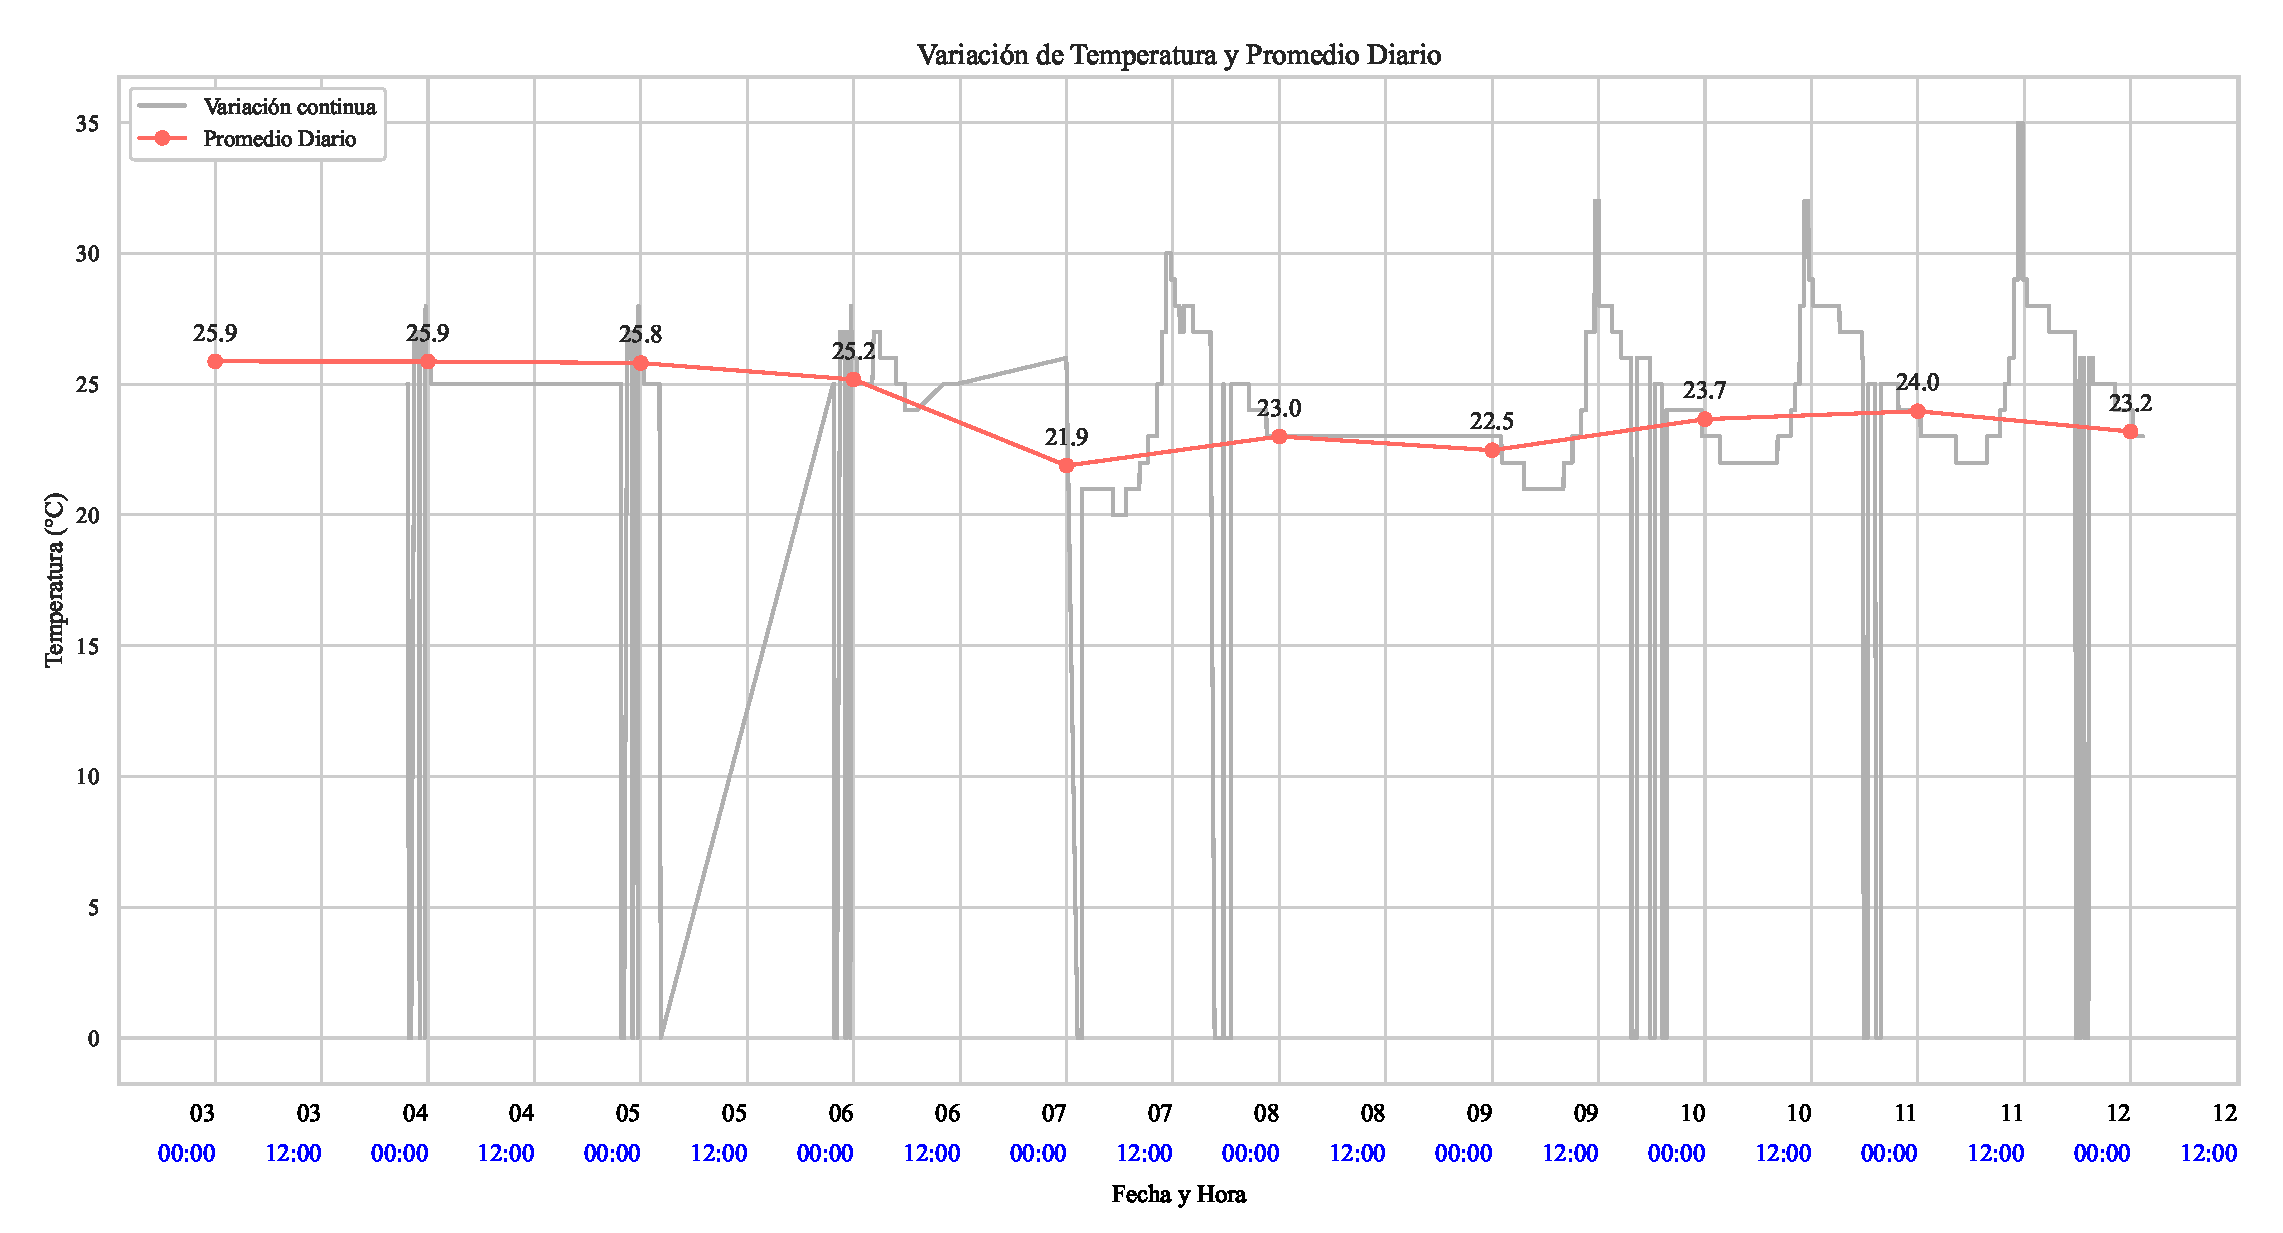
\includegraphics[width=0.8\textwidth]{assets/temperatura_continua_y_promedio.eps}
    \caption{Variación y promedio diario de la temperatura ambiente durante el periodo experimental.}
    \label{fig:temperatura_promedio}

    \vspace{0.4cm}

    \noindent
    \begin{minipage}[t]{0.49\textwidth}
        \justifying
         En el transcurso del periodo experimental, el asistente de riego registraba el valor de la temperatura ambiente mediante un sensor de temperatura que se describe en el apartado de Métodos. En la figura \ref{fig:temperatura_promedio}, se muestra un rango de los valores registrados que va desde los 0°C hasta los 35°C con un comportamiento irregular y discontinuo.

        Este rango de 35 unidades se debe en mayor parte a la inaccesibilidad del módulo de recolección de datos a los valores recopilados por el módulo de riego,

    \end{minipage}%
    \hfill
    \begin{minipage}[t]{0.49\textwidth}
        \justifying
        \noindent ocasionando descensos abruptos a los 0°C. Aunado a esto, no se tiene registro de la variabilidad de la temperatura en dos periodos: del 5 de junio, desde la 01:00 hasta las 22:00 horas, y del 6 de junio, desde las 00:00 hasta las 12:00 horas.

        Esta ausencia de valores registrados se debe, en mayor parte, a problemas en la implementación inicial del asistente, lo que ocasionó que, inicialmente, el sistema haya tomado decisiones sin considerar la temperatura con la relevancia para la que fue diseñado.   
	\end{minipage}

    \vspace{0.5cm}
    %\caption{Temperatura promedio registrada durante el experimento}
    \hrule
\end{figure}

\begin{figure}[!ht]
    \centering
    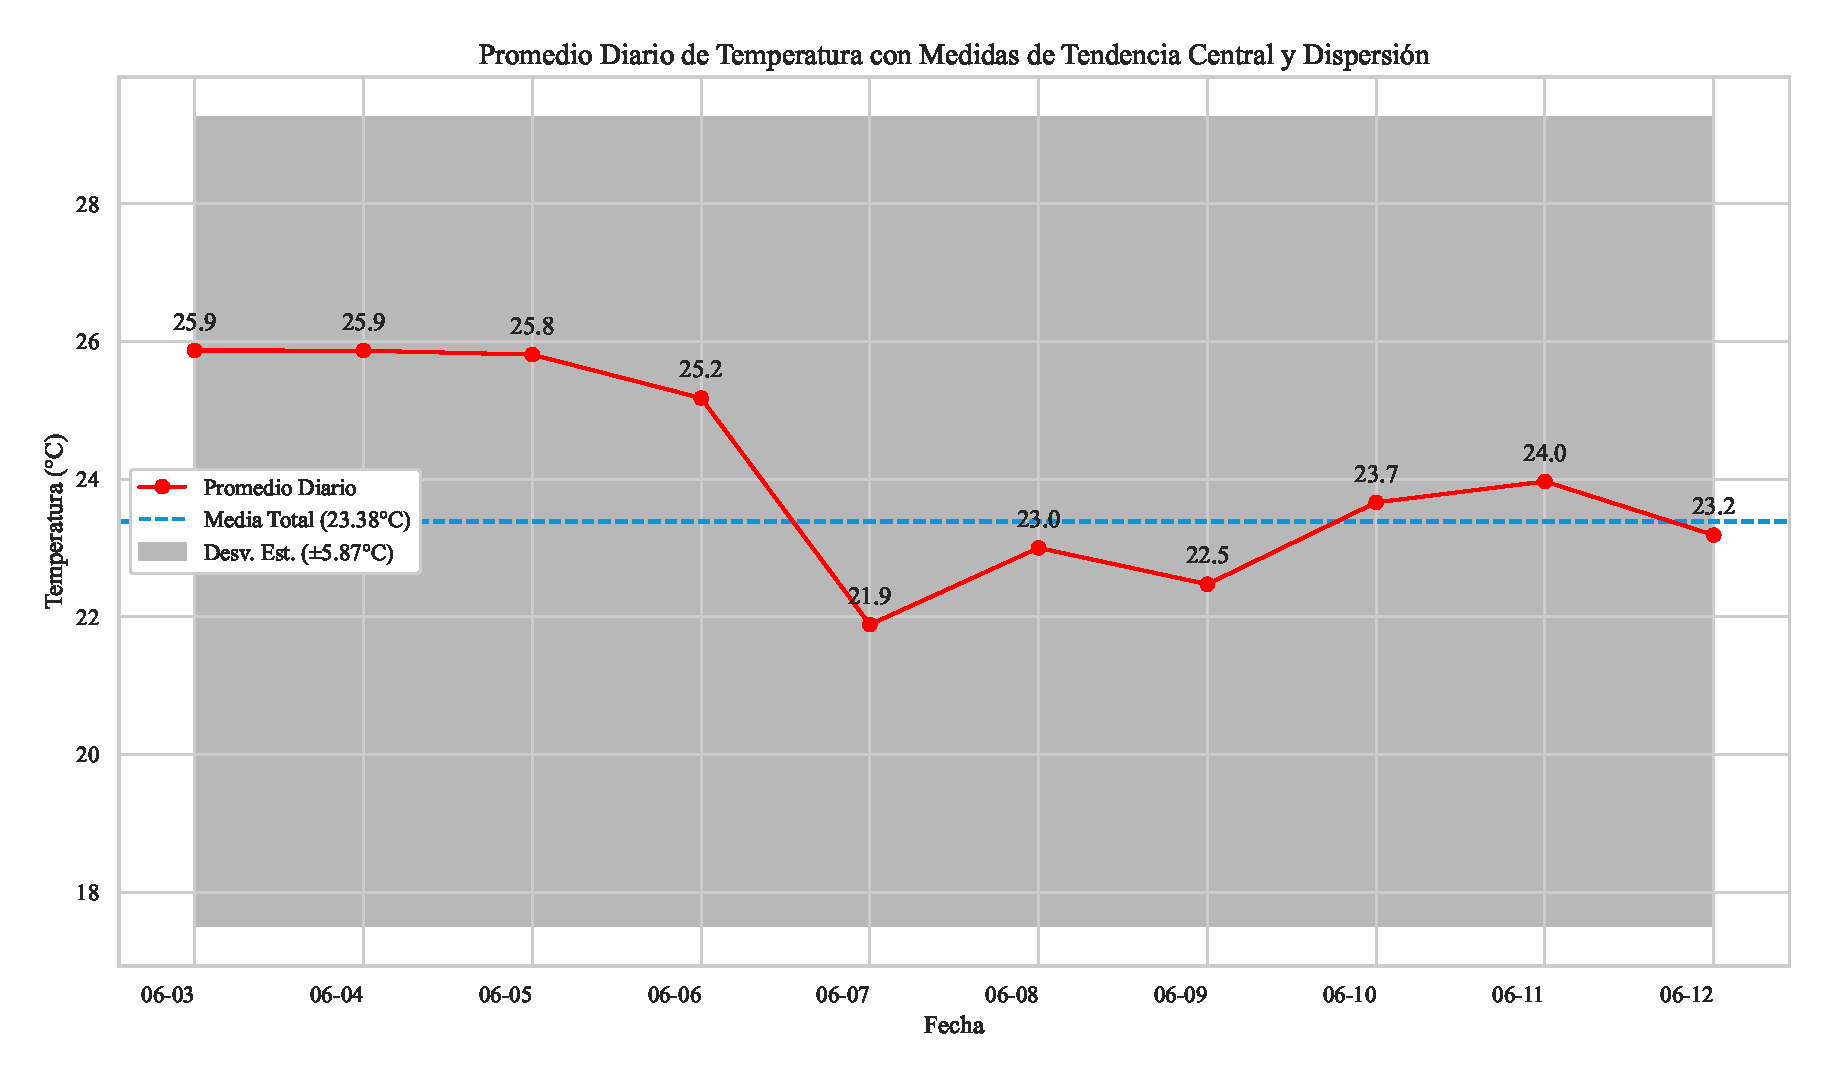
\includegraphics[width=1\textwidth]{assets/temperatura_promedio_y_estadisticas.eps}
    \caption{Promedio diario, promedio total y dispersión de la temperatura ambiente durante el periodo experimental.}
    \label{fig:temperatura_desviacion}

    \vspace{0.4cm}

    \noindent
    \begin{minipage}[t]{0.45\textwidth}
        \justifying
        En la figura \ref{fig:temperatura_desviacion} se muestran los promedios diarios de temperatura, la media total de 23.38°C y la dispersión de $\pm$5.87°C de todos los registros de temperatura recopilados. Estos datos son relevantes para comprender el comportamiento del asistente de riego.
	\end{minipage}%
    \hfill
    \begin{minipage}[t]{0.45\textwidth}
        \justifying
        El promedio de los primeros tres días se mantuvo constante debido a la invariabilidad de las lecturas, sin embargo, hubo un descenso del 5 al 7 de junio al valor medio diario más bajo del periodo de estudio. Posteriormente, la temperatura ascendió en el resto del periodo hasta una media de 24°C.

\end{minipage}

    \vspace{0.5cm}
    \hrule
    %\caption{Temperatura promedio registrada durante el experimento}
\end{figure}

\begin{multicols}{2}
\justifying
%%--------------------------------
El periodo que mejor refleja el comportamiento de la temperatura comprende del 9 hasta el 12 de junio, donde se puede observar el siguiente patrón si se omiten los datos donde la temperatura es de 0°C: diariamente, las temperaturas más altas se registran al mediodía, mientras que los valores más bajos se observan entre la medianoche y el mediodía. 

Con esto, se puede indicar que el asistente contó con valores más congruentes con el estado del jardín doméstico, especialmente desde el 9 de junio, adaptándose mejor a las condiciones como se discute en el apartado de consumo de agua.

Además de la temperatura, \cite{ref12} menciona la humedad como la principal variable neccesaria para monitorear la retención de agua en la tierra de los jardines domésticos. Por eso, en el siguiente apartado, se discuten los valores obtenidos al vigilar las vaariaciones de este fenómeno en el espacio de estudio.
\subsection*{Monitoreo de humedad}

La humedad promedio del suelo, medida durante el período de estudio de 10 días, oscila entre 707.25 y 802.83 unidades en una escala de 0 (presencia total de humedad) a 4500(ausencia total de humedad) establecida por el sensor de humedad implementado dentro del sistema de riego según los datos registrados.

Los primeros días del periodo se identifican como una fase de calibración y adaptación inicial del sistema de riego. Durante este periodo inicial se obtienen valores más altos de humedad como se muestra en la Figura~\ref{fig:humedad_del_suelo}.

Al pasar el cuarto día, los valores se van normalizando hasta lograr una tendencia uniforme por el resto del periodo, siendo reflejado en la frecuencia de riego por día, mostrando la adaptación del sistema a su entorno al reducir la frecuencia.  

Si bien un periodo de observación más extenso permitiría identificar esta tendencia, los resultados actuales ya evidencian una mejora significativa en la capacidad del sistema para mantener condiciones de humedad constantes, lo cual es fundamental para la optimización del consumo de agua en entornos domésticos que será explorada a detalle en la siguiente sección.
\end{multicols}
\newpage
\begin{figure}[!ht]
    \centering
    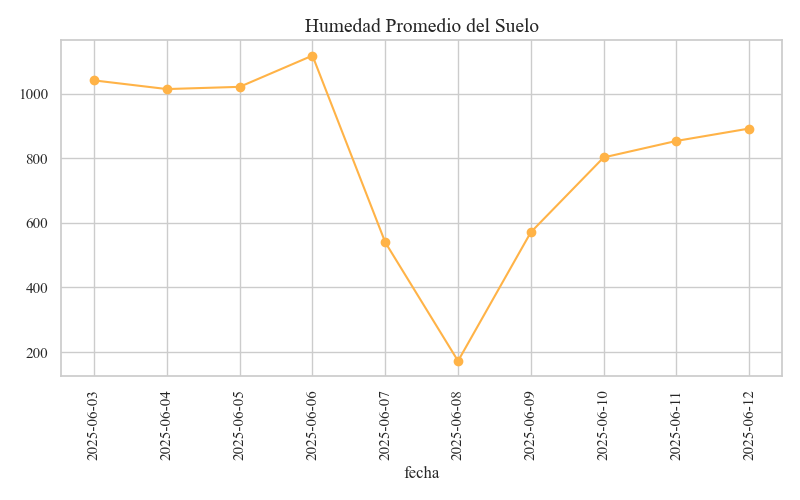
\includegraphics[width=1\textwidth]{assets/humedad_promedio.png}

    \caption{Humedad promedio registrada durante el periodo experimental}
    \label{fig:humedad_del_suelo}

    \vspace{0.4cm}

    \noindent
    \begin{minipage}[t]{0.49\textwidth}
        \justifying
        Esta figura muestra la evolución promedio de la humedad registrada por los sensores en el jardín doméstico durante el periodo.

        Muestra el proceso de normalización de la humedad
    \end{minipage}%
    \hfill
    \begin{minipage}[t]{0.49\textwidth}
        \justifying
        \noindent del suelo del jardín doméstico. Con valores altos en los primeros días indicando poca humedad en el suelo, para, posteriormente, pasar por un día de sobreirrigación y finalmente mantener valores dentro del mismo rango.
    \end{minipage}

    \vspace{0.5cm}
    \hrule
\end{figure}

\begin{multicols}{2}
\justifying
%%--------------------------------

\subsection*{Consumo de agua}
Durante los 10 días de monitoreo de la fase de implementación del asistente inteligente de riego se registraron 2 días cuya frecuencia de riego fue de dos veces. Posteriormente, cada dos días se regaba una vez. Esto se puede ver en la figura \ref{fig:activaciones_riego_diarias}.

En la figura \ref{fig:activaciones_riego_dispersion} se puede contemplar que la media general de frecuencia de riego fue de 0.8 veces, sin embargo, ya que hubo una dispersión de $\pm$0.79, aún se necesitó de más tiempo de aplicación para reducir esta dispersión y obtener un promedio de actividades de riego más preciso.

Considerando que, por cada apertura de las válvulas, se daba el paso a 4.93 L; en los primeros dos días se hizo un gasto diario de 9.86 L; luego, el gasto se redujo a 4.93 L por cada dos días. Esto se puede notar en la figura \ref{fig:consumo}.

De igual forma, en la figura \ref{fig:consumo_estadisticas} se puede observar que, considerando el mismo volumen consumido por cada activación de las válvulas, se hizo un consumo medio de 3.94 L con una desviación estándar de 3.89 L. Tal como en la dispersión de la frecuencia de activaciones de las válvulas para regar el jardín, la dispersión con una magnitud absoluta similar a la media indica que los datos están muy dispersos y que, si se continuara por un periodo más extenso de estudio, se podrían obtener datos más precisos.. 

En comparación, el sistema de riego tradicional tiene una frecuencia de riego de una vez al día en un horario fijo con el ajuste manual del volumen de riego ante la presencia de lluvia a lo largo del día, consumiendo 78 L para un periodo equivalente. Estos resultados y datos recabados se discuten en la siguiente sección.

%%----------- Figura ------------
\end{multicols}
\begin{figure}[!h]
    \centering
    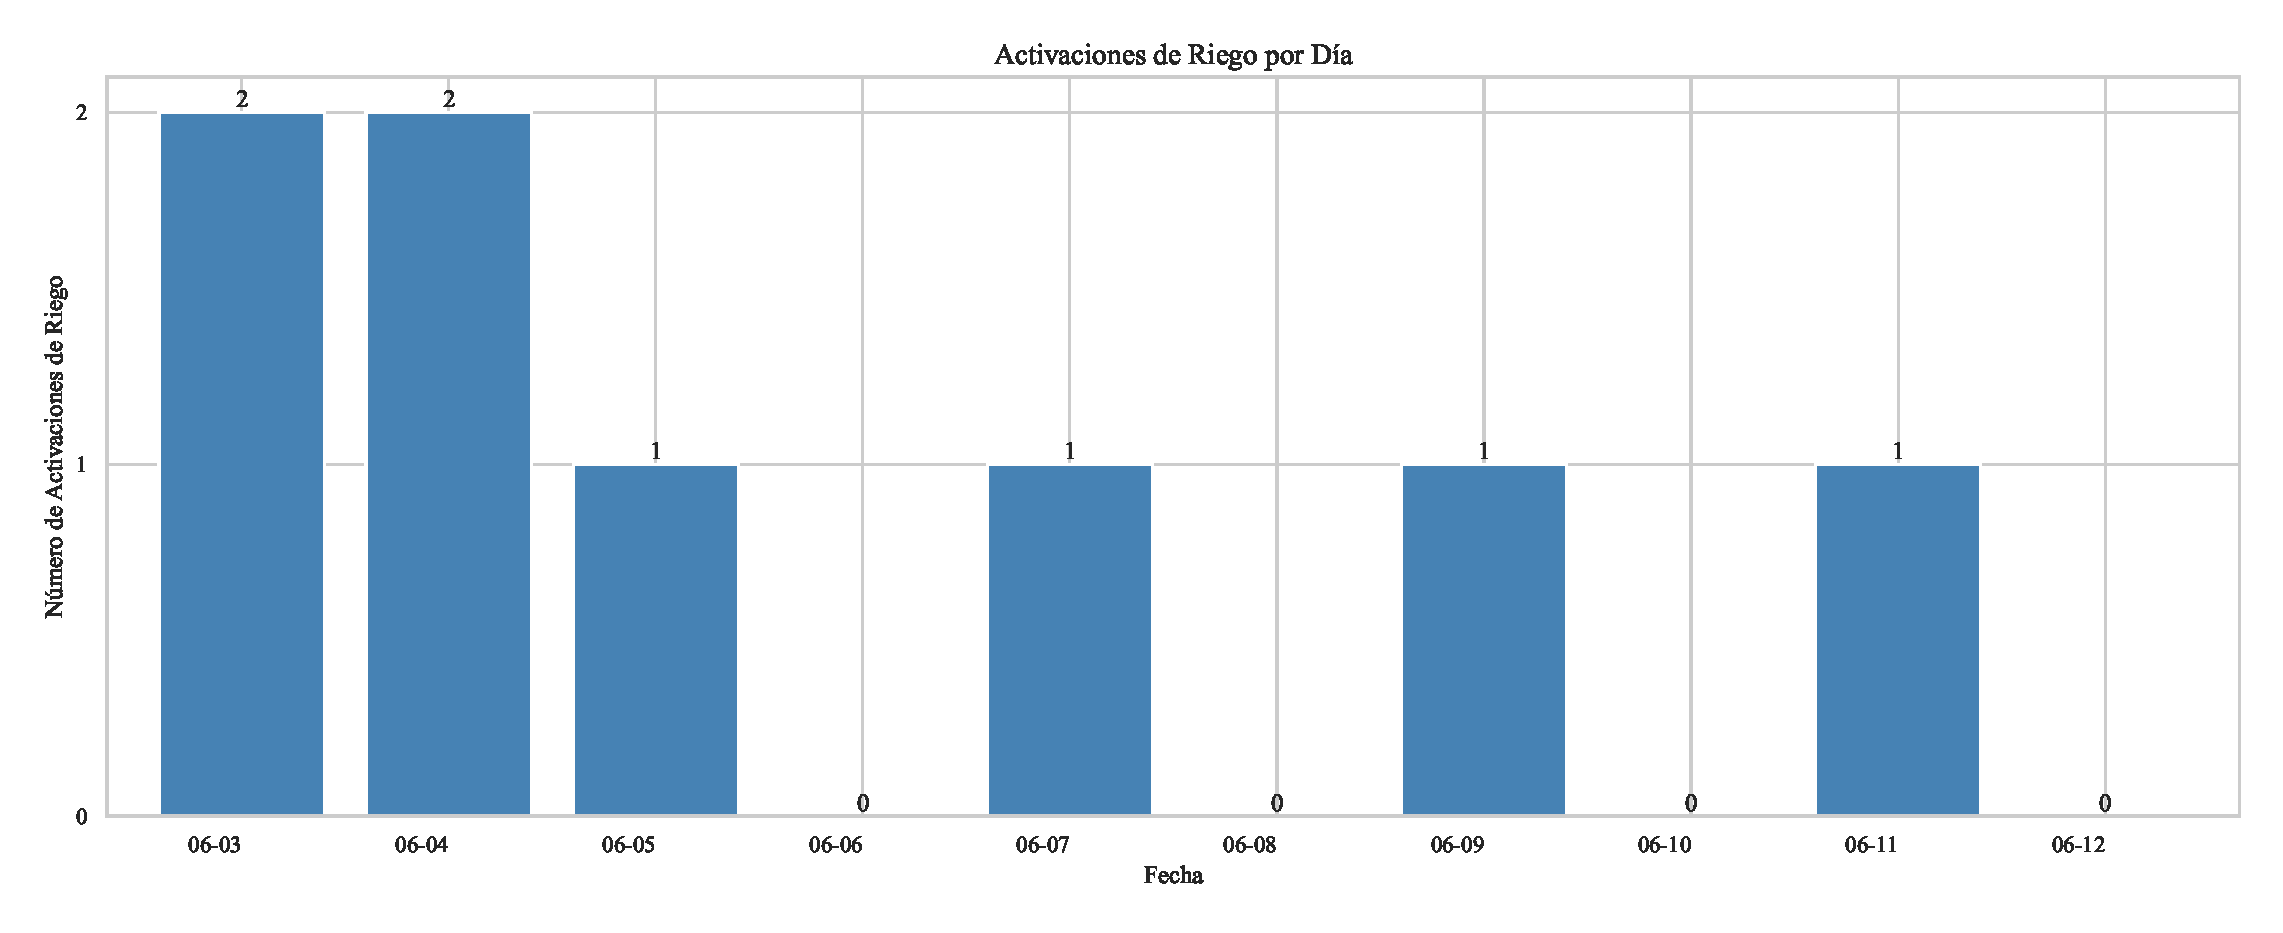
\includegraphics[width=1\textwidth]{assets/activaciones_riego_diarias.eps}
    \caption{Activaciones de riego diaria durante el periodo experimental.}
    \label{fig:activaciones_riego_diarias}

    \vspace{0.4cm}

    \noindent
    \begin{minipage}[t]{0.45\textwidth}
        \justifying
	\end{minipage}%
    \hfill
    \begin{minipage}[t]{0.45\textwidth}
        \justifying

\end{minipage}

    \vspace{0.5cm}
    \hrule
    %\caption{Temperatura promedio registrada durante el experimento}
\end{figure}

\newpage

\begin{figure}[!ht]
    \centering
    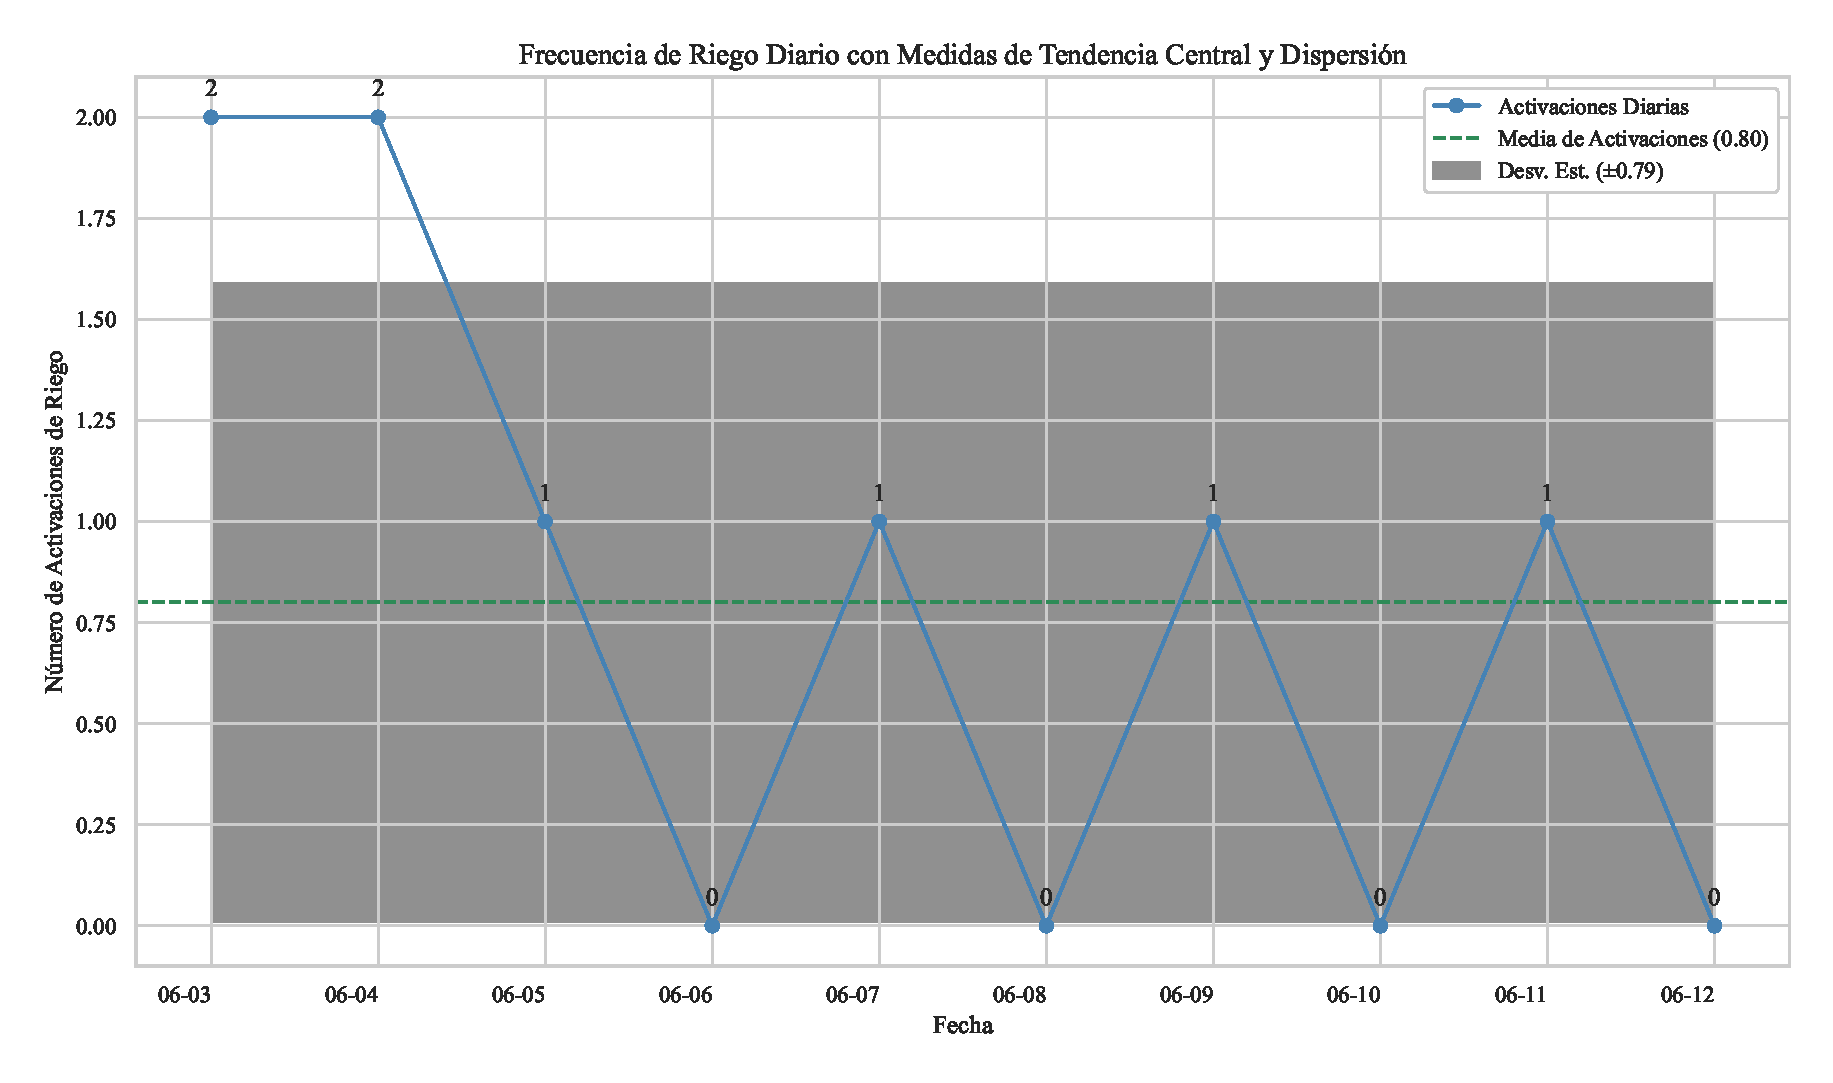
\includegraphics[width=1\textwidth]{assets/activaciones_riego_promedio_y_estadisticas.eps}
    \caption{Promedio de activaciones de riego, media general y dispersión de la frecuencia de riego durante el periodo experimental.}
    \label{fig:activaciones_riego_dispersion}

    \vspace{0.4cm}

    \noindent
    \begin{minipage}[t]{0.45\textwidth}
        \justifying
	\end{minipage}%
    \hfill
    \begin{minipage}[t]{0.45\textwidth}
        \justifying

\end{minipage}

    \vspace{0.5cm}
    \hrule
    %\caption{Temperatura promedio registrada durante el experimento}
\end{figure}
\begin{multicols}{2}
\justifying
%%--------------------------------
\end{multicols}


\begin{figure}[!ht]
    \centering
    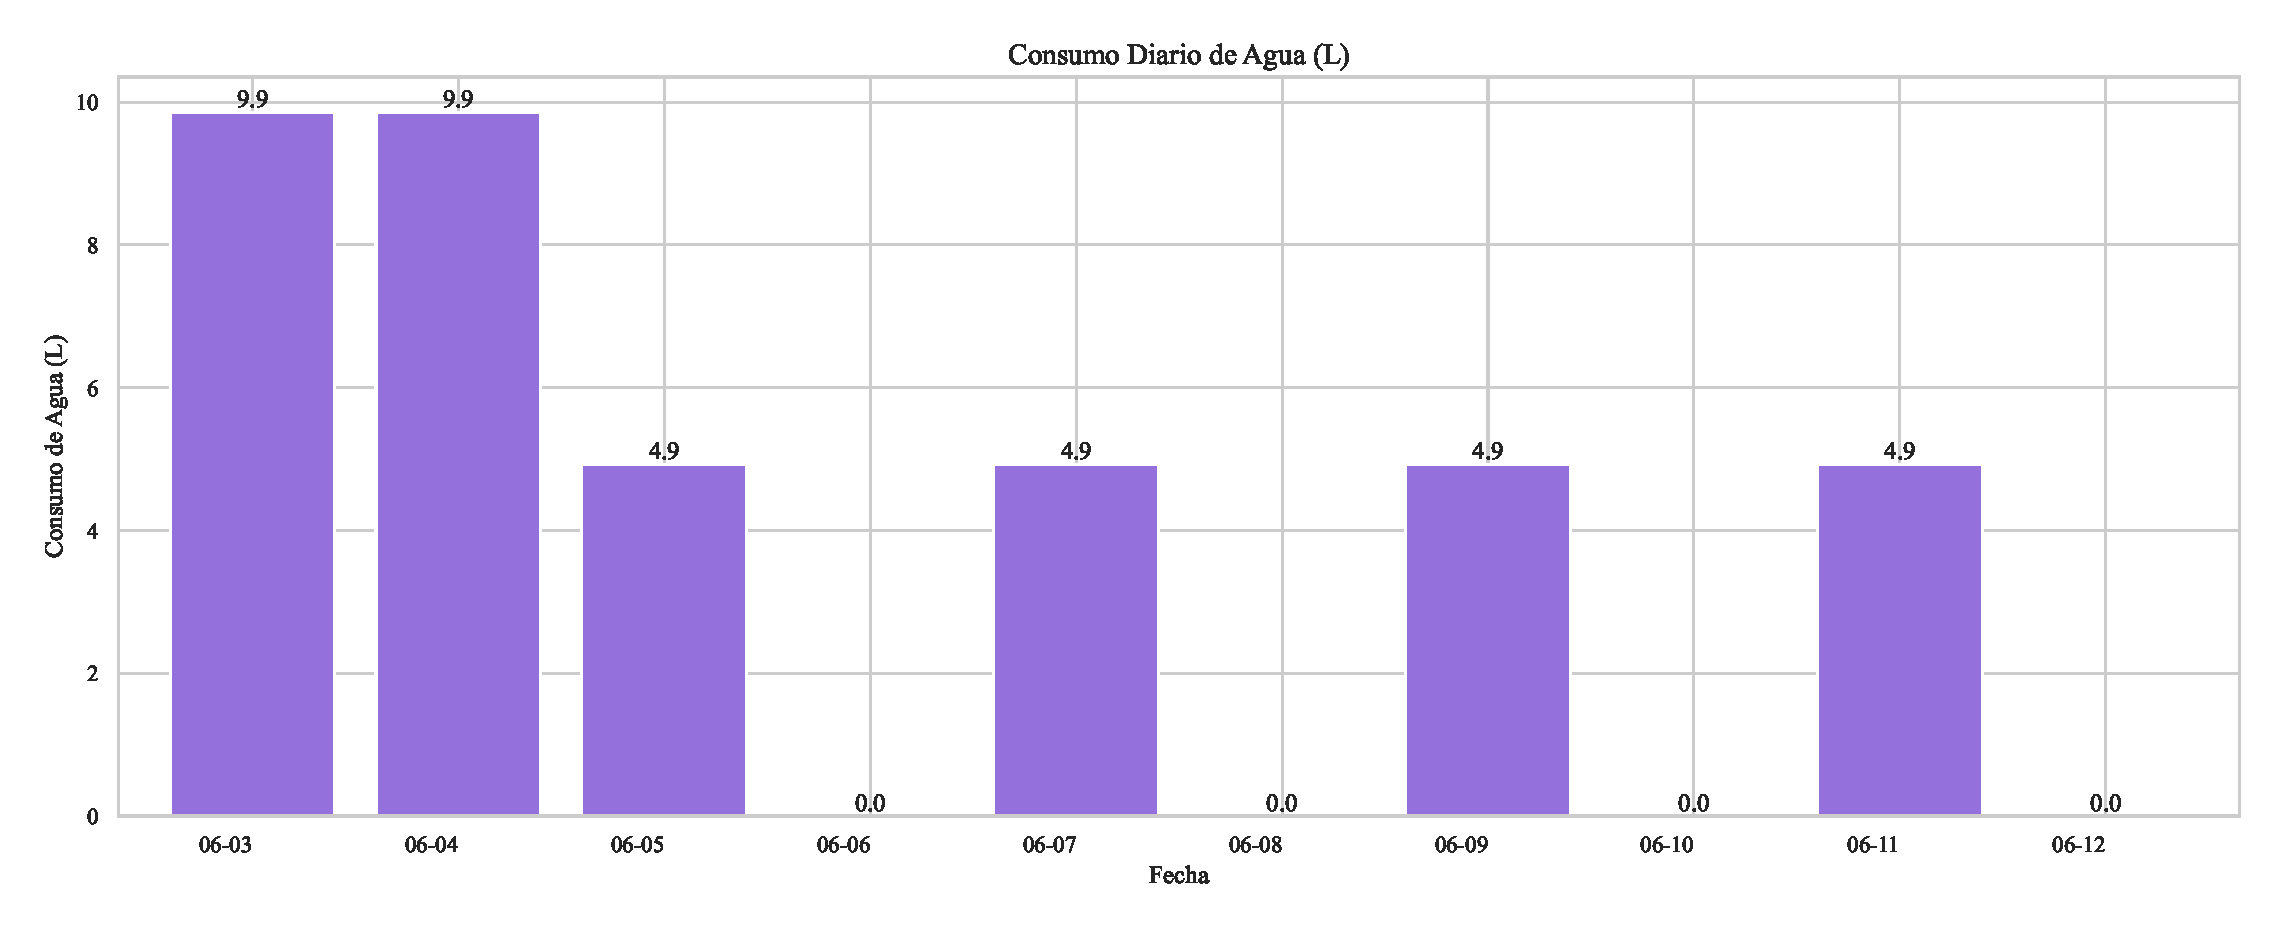
\includegraphics[width=1\textwidth]{assets/consumo_diario_barras.eps}

    \caption{Consumo diario de agua durante el periodo experimental}
    \label{fig:consumo}

    \vspace{0.4cm}

    \noindent
    \begin{minipage}[t]{0.48\textwidth}
        \raggedright
        Esta figura muestra el uso del agua durante el periodo experimental de este proyecto.
    \end{minipage}
    \hfill
    \begin{minipage}[t]{0.48\textwidth}
        \justifying
        En esta figura se observa cómo fue reduciéndose el consumo de agua por día, mostrando el ajuste del sistema de riego a las necesidades del jardín.
    \end{minipage}

    \vspace{0.5cm}
    \hrule
\end{figure}

\begin{multicols}{2}
\justifying
%%--------------------------------

%%----------- Figura ------------
\end{multicols}
\begin{figure}[!ht]
    \centering
    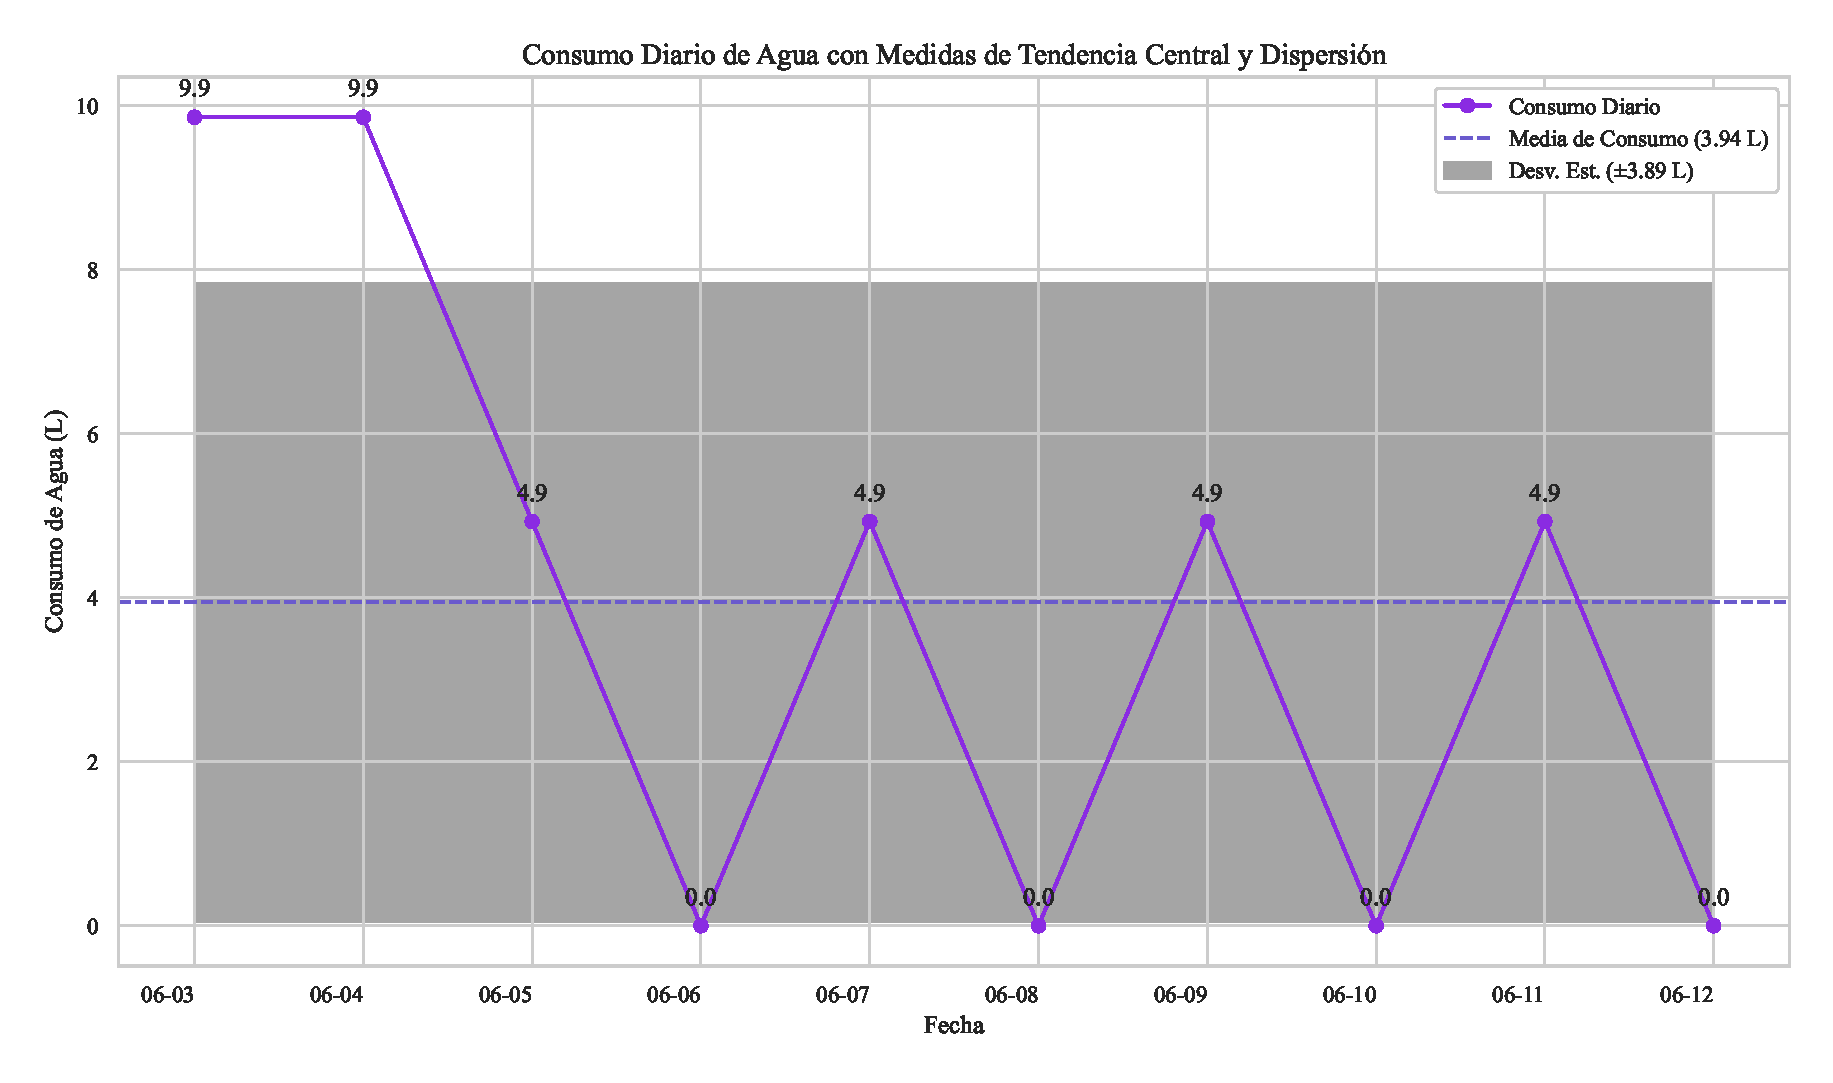
\includegraphics[width=1\textwidth]{assets/consumo_diario_promedio_y_estadisticas.eps}
    \caption{Promedio diario, promedio total y dispersión del consumo de agua durante el periodo experimental.}
    \label{fig:consumo_estadisticas}

    \vspace{0.4cm}

    \noindent
    \begin{minipage}[t]{0.45\textwidth}
        \justifying
	\end{minipage}%
    \hfill
    \begin{minipage}[t]{0.45\textwidth}
        \justifying

\end{minipage}

    \vspace{0.5cm}
    \hrule
    %\caption{Temperatura promedio registrada durante el experimento}
\end{figure}
\newpage

\begin{multicols}{2}
\justifying
%%--------------------------------

\section*{Discusión}

\subsection*{Reducción en el consumo de agua}

El asistente inteligente de riego demostró una reducción significativa en el consumo de agua en un periodo de 10 días, el sistema tradicional consumió un aproximado de 78 L mientras que el sistema propuesto, tuvo un consumo total de aproximadamente 39.44 L en un periodo igual a 10 días como se menciona en la sección de resultados. Esto representa una notable reducción del 49.44\%. Este hallazgo valida la capacidad del sistema para optimizar el uso del agua en entornos domésticos, lo que se traduce en ahorro económico y una importante contribución a la sostenibilidad hídrica. Los resultados obtenidos se encuentran en el rango de las expectativas de reducción de consumo de agua esperadas del 30\% a 50\% atribuidas a sistemas inteligentes de IA, demostrando una alta eficiencia para una solución adaptable al contexto doméstico y de bajo costo.

La principal limitación es el corto periodo de monitoreo de 10 días, que, aunque muestra buenos resultados, requiere validación a largo plazo para que pueda considerar más cambios de clima como, por ejemplo días constantes de lluvia o soleados o fríos y de ese modo tener una identificación de patrones estacionales que podrían influir en el consumo. A pesar de eso, el éxito del sistema resalta muy bien el potencial del machine learning en sistemas embebidos para la optimización de recursos, sin embargo, se tendrá contemplado que para futuras investigaciones se deberá extender el tiempo de monitoreo.

\subsection*{Variables relevantes}
El monitoreo de variables ambientales que también se hace mención en la sección de resultados fue fundamental para el funcionamiento del sistema, se encontró una correlación positiva moderada entre la temperatura ambiente y la frecuencia de riego, con temperaturas diarias promedio de 23.38°C, sin embargo, se identificaron dos casos atípicos de riego en las temperaturas de 0°C y 26°C, con respecto a la humedad del suelo, los valores oscilaron entre 707.25 y 802.83 unidades, y también, se evidenció una fase inicial de calibración con valores de humedad más altos, seguida de una normalización y una tendencia uniforme a partir del cuarto día, lo que se correlacionó con una reducción en la frecuencia de riego.

La correlación positiva entre la temperatura y la frecuencia de riego es un indicador crucial de que el sistema responde de manera lógica a las necesidades hídricas del jardín, los casos atípicos nos muestran áreas para la mejora en la robustez del modelo frente a valores extremos o lecturas inusuales y el comportamiento de la humedad del suelo demuestra la capacidad de adaptación y autorregulación del sistema. Esta fase de calibración inicial es esperable en un sistema de machine learning que se adapta al entorno, se ajustó y mantuvo la humedad del suelo en un nivel ideal, lo que automáticamente redujo la frecuencia de riego, eso válida la eficiencia del algoritmo para evitar el sobre-riego y garantizar el suministro adecuado de agua.

Similar al consumo de agua, la limitación principal fue el periodo de monitoreo de solo 10 días, que, aunque suficiente para observar tendencias iniciales y la adaptación del sistema, no permite capturar variaciones estacionales en la temperatura y la humedad, las cuales sí pudieron haber influido en el rendimiento del sistema. La presencia de casos atípicos en la temperatura también nos muestra que el modelo podría beneficiarse de algoritmos más avanzados para el manejo de valores extremos.

El sistema mostró que puede mantener la salud del jardín mientras se minimiza el desperdicio de agua. En futuras investigaciones se podría poner más enfoque en la integración de más variables fuera de los sensores como lo son los pronósticos meteorológicos a corto plazo. También sería valioso explorar la implementación de algoritmos de machine learning más complejos que puedan aprender patrones a largo plazo y manejar de forma más sofisticada los datos atípicos para optimizar aún más la toma de decisiones de riego.
\section*{Métodos}

\subsection*{Componentes usados}

El sistema de riego inteligente fue diseñado con una arquitectura modular basada en el microcontrolador ESP32-WROOM-32 (Expressif Systems), por su conectividad Wi-Fi integrada y soporte para protocolos de comunicación inalámbrica de baja latencia, como ESP-NOW, que permite la interoperabilidad sin conexión constante a internet (Ponce Pérez et al., 2021). 

La arquitectura incluye sensores ambientales, una unidad de procesamiento y actuadores, componentes interconectados para monitorear y controlar el riego en tiempo real en un jardín doméstico experimental.

Los siguientes componentes fueron integrados, con especificaciones técnicas para garantizar el rendimiento y la compatibilidad:
\begin{itemize}
  \item Microcontrolador ESP32-WROOM-32: Placa de desarrollo con ADC (Convertidor Analogico-Digital) de 12 bits, 32 pines GPIO (pins de Entrada y salida de Propósito General) digitales/analógicos y soporte para Micro Python. Se conectó a sensores a través de pines ADC (GPIO 34 para salida analógica, GPIO 32 para salida digital) y GPIO digitales (GPIO 15 para el relé). Su capacidad de procesamiento permite ejecutar algoritmos de decisión en tiempo real\cite{ref5}.
  \item Sensor de Humedad YL-69/YL-38: Un sensor resistivo de humedad del suelo (YL-69) acoplado al módulo YL-38, que incluye un comparador LM393 SMD. El módulo YL-38 ofrece salidas analógica (A0, 0-4.2 V) y digital (D0, ajustable por umbral). Especificaciones: voltaje de operación 3.3-5 V, corriente 35 mA. La salida analógica A0 se conectó al pin GPIO 34 del ESP32 para lecturas de contenido volumétrico de agua (VWC). Debido a su diseño resistivo, se reconoce la limitación por corrosión a largo plazo \cite{ref6}.
  \item Sensor de Temperatura y Humedad DHT11: Sensor digital que mide temperatura (0-50°C, precisión $\pm$2°C, resolución 0.1°C) y humedad del aire (20-90\% RH, precisión $\pm$4\% RH, resolución 1\% RH). Opera a 3.3-5 V y se conecta al GPIO 32 del ESP32 mediante una interfaz de un solo cable para salida digital \cite{ref7}. 
  \item Sensor de Lluvia: Módulo basado en el comparador LM393, con una celda de detección. Opera a 3.3-5 V y proporciona una salida analógica (conectada al pin GPIO 35 del ESP32) y digital (D0, ajustable). Detecta precipitaciones para inhibir el riego, con un tiempo de respuesta $<$1 s \cite{ref8}.
  \item Electroválvula Solenoide: Válvula de 3/4'' NPS, normalmente cerrada (NC), fabricada en plástico y latón, con voltaje de actuación de 12 VDC, corriente de 300 mA, presión de trabajo de 0.02-0.8 MPa y vida útil de 50,000 ciclos. Se conectó a través de un relé al pin GPIO 15 del ESP32, permitiendo el control del flujo de agua con tiempos de respuesta de 0.15 s (apertura) y 0.3 s (cierre) \cite{ref9}.
  \item Relé: Módulo de relé estándar de 12 V, con un canal de control a 5 V, conectado al pin GPIO 15 del ESP32 para activar la electroválvula. Soporta corrientes de hasta 10 A, asegurando una actuación confiable \cite{ref10}.
  \item Fuente de Alimentación: Fuente regulada de 5V DC, 2 A, implementada mediante un convertidor reductor (modelo LM2596) para alimentar el ESP32, sensores y relé. La electroválvula se alimentó con una fuente separada de 12 VDC, 1 A, para evitar interferencias \cite{ref11}.
\end{itemize}

Los componentes se ensamblan en una carcasa resistente a la intemperie, con cables de sensores expuestos al suelo y la atmósfera. Las conexiones se realizaron mediante una placa de prototipado, con los pines del ESP32 asignados como sigue: GPIO 34 (A0 del YL-38), GPIO 32 (DHT11), GPIO 35 (A0 del sensor de lluvia), GPIO 15 (relé para electroválvula).

El firmware del ESP32 se desarrolló en MicroPython utilizando el IDE Thonny, con las bibliotecas machine para control de pines como dht para el DHT11 y utime para sincronización. 

El algoritmo de control implementó una lógica basada en umbrales: el riego se activa si la humedad del suelo (lectura analógica del YL-38) cae por debajo del 40% VWC, la temperatura (DHT11) supera 25°C y no se detecta lluvia (sensor de lluvia, salida digital D0 en bajo). 

Los eventos de riego se limitan a 1-2 minutos, con un máximo de 4 eventos diarios. Los datos de sensores se procesan cada 30 minutos, con filtrado de ruido mediante un promedio móvil (ventana de 5 muestras).

\subsection*{Distribución de asistente inteligente de riego}
La arquitectura funcional del sistema se diseñó siguiendo el enfoque de tres capas descrito anteriormente: percepción, procesamiento y actuación. Esta estructura se implementó mediante tres módulos físicos: el módulo de recolección de datos, el módulo de procesamiento y el módulo de válvulas, cada uno con funciones específicas coordinadas a través de comunicación inalámbrica directa.

El módulo de recolección de datos está conformado por sensores encargados de medir la humedad del suelo, temperatura ambiental y la presencia de lluvia, permitiendo capturar en tiempo real las condiciones ambientales del entorno de prueba.

Los datos obtenidos se transmiten al módulo de procesamiento utilizando el protocolo ESP-NOW, que permite la comunicación entre microcontroladores sin necesidad de conexión a internet o infraestructura adicional.

El módulo de procesamiento actúa con los datos recopilados por el anterior módulo. Este módulo ejecuta un modelo de regresión logística, cuyo objetivo es predecir la necesidad de riego en función de las variables ambientales medidas. 

La decisión de activar el riego se basa en la probabilidad estimada por el modelo, utilizando un umbral de activación ajustado a un valor de 0.5, si la predicción del modelo sobrepasa el umbral mencionado se regará el jardín en caso contrario no se llevará a cabo el riego. 

Finalmente, el módulo de válvulas implementa la capa de activación del sistema. A partir de la señal emitida por el módulo de procesamiento, este módulo opera una electroválvula mediante un circuito de control con relé, permitiendo el paso de agua al jardín cuando las condiciones lo requieren. 

Esta estructura modular y distribuida facilita la expansión del sistema a mayor escala mediante la replicación de nodos sensores, manteniendo una lógica de control centralizada.

\section*{Recopilación de datos}

El sistema fue evaluado durante un periodo experimental de diez días comprendido entre el 3 y el 12 de junio de 2025. Durante este intervalo, se registraron de forma continua las siguientes variables: humedad del suelo, temperatura ambiental, ocurrencia de lluvia y activaciones de la electroválvula. Los datos fueron almacenados localmente en formato CSV dentro de la memoria no volátil, con el objetivo de facilitar su posterior análisis fuera de línea.

Para realizar la consulta de los datos almacenados, el proceso de medición se interrumpe en un periodo de 10 minutos, lo cual hacía que se perdieran datos del jardín en este tiempo. Sin embargo, no se interrumpe el accionamiento de las válvulas, además de que estas interrupciones se realizaban en horarios que no interfirieran en el funcionamiento del módulo de procesamiento.

La frecuencia de muestreo no fue constante, ya que estuvo determinada por la lógica de activación del microcontrolador y el comportamiento dinámico de las condiciones ambientales. A pesar de esta variabilidad, los datos obtenidos resultaron suficientes para construir series temporales que permitieron analizar tendencias de comportamiento del sistema. 

El análisis exploratorio de los datos fue realizado externamente mediante herramientas de hoja de cálculo y análisis de datos en Python, lo que permitió identificar patrones de estabilización del sistema, así como inferir su capacidad de adaptación progresiva al entorno específico en el que fue implementado.

\section*{Conclusión}

En un periodo de 10 días, se logró una notable reducción del 49.44\% en el consumo de agua comparado con el riego tradicional, este hallazgo no solo confirma que el sistema es capaz de generar ahorros económicos directos para la persona que lo use, sino que también válida su potencial para contribuir a la sostenibilidad hídrica en el ámbito residencial y a las investigaciones en el ámbito tecnológico. La efectividad del sistema se fundamenta en su capacidad para monitorear variables ambientales clave como la temperatura y la humedad del suelo, adaptando la frecuencia de riego de manera inteligente para evitar el sobre-riego y garantizar el suministro adecuado de agua.

Si bien el periodo de monitoreo de pocos días representa una limitación para identificar patrones estacionales a largo plazo y las condiciones del sistema a condiciones climáticas extremas, el estudio valida la eficiencia del algoritmo y la robustez del diseño. Este trabajo, adicionalmente, contribuye al campo al ofrecer una solución práctica, de bajo costo y adaptada al contexto doméstico, cerrando la brecha existente en el mercado. Para futuras investigaciones, se plantea la extensión del periodo de monitoreo y la integración de pronósticos meteorológicos para una gestión más predictiva.

\section*{Disponibilidad de datos}
Para acceder a los datos de entrenaiento del modelo utilizado en este proyecto puede acceder a este enlace donde encontrará un archivo CSV que le ayudará a entrenar el modelo para realizar predicciones sobre el jardín en el que se desee implementar \url{https://github.com/BraveHunt25/asistente-inteligente-de-riego/tree/main/Datos}

\section*{Disponibilidad de código}
Para consultar el código utilizado en la implementación de este sistema de riego inteligente puede acceder al siguiente repositorio \url{https://github.com/BraveHunt25/asistente-inteligente-de-riego}, donde encontrará el código para cada uno de los módulos del sistema de riego, el módulo emisor, el módulo de procesamiento y el módulo de control de las válvulas.
%%===========================================================================================%%
%% If you are submitting to one of the Nature Portfolio journals, using the eJP submission   %%
%% system, please include the references within the manuscript file itself. You may do this  %%
%% by copying the reference list from your .bbl file, paste it into the main manuscript .tex %%
%% file, and delete the associated \verb+\bibliography+ commands.                            %%
%%===========================================================================================%%

%%===========================================================================================%%
%% The following content was generated by BibTeX and is now embedded directly.               %%
%% You may need to compile twice to see the citations correctly numbered.                    %%
%%===========================================================================================%%
\begin{thebibliography}{4}


\bibitem{ref1}
Organización de las Naciones Unidas.
\textit{Objetivo 11: Lograr que las ciudades sean más inclusivas, seguras, resilientes y sostenibles}.
Organización de las Naciones Unidas, 2023.
[En línea]. Disponible en: \url{https://www.un.org/sustainabledevelopment/es/water-and-sanitation/}.
[Último acceso: 21 06 2025].

\bibitem{ref2}
E. Vega López.
\textit{Agua, crecimiento económico y bienestar social en México}.
Revista de Economía Mexicana Anuario UNAM, vol. I, no. 8, pp. 233–294, 2023.

\bibitem{ref3}
A. Glória, J. Cardoso y P. Sebastiäo.
\textit{Sustainable Irrigation System for Farming Supported by Machine Learning and Real-Time Sensor Data}.
Sensors, 2021.

\bibitem{ref4}
Comisión del Agua del Estado de México.
\textit{Tarifas de agua potable, drenaje y tratamiento de aguas residuales}.
Agencia Digital del Estado de México, 2024.
[En línea]. Disponible en: \url{https://caem.edomex.gob.mx/tarifas_agua_potable_drenaje_y_tratamiento_aguas_residuales}.
[Último acceso: 21 06 2025].


\bibitem{ref5}
Espressif.
\textit{Ficha técnica del Microcontrolador ESP32}
Espressif Systems, 2025.
[En línea]. Disponible en:\url{https://www.espressif.com/sites/default/files/documentation/esp32-wroom-32_datasheet_en.pdf}
[Último acceso: 24 06 2025] 

\bibitem{ref6}
Texas Instruments.
\textit{Ficha técnica Sensor de Humedad YL-69}
Texas Instruments, 2025.
[En línea]. Disponible en:\url{https://www.ti.com/lit/ds/symlink/lm393-n.pdf}
[Último acceso: 24 06 2025] 

\bibitem{ref7}
AOSONG.
\textit{Ficha técnica Sensor de Temperatura y Humedad DHT11}
APSONG Electronics, 2025.
[En línea]. Disponible en:\url{https://components101.com/sites/default/files/component_datasheet/DFR0067%20DHT11%20Datasheet.pdf}
[Último acceso: 24 06 2025] 

\bibitem{ref8}
STMicroelectronics.
\textit{Ficha técnica comparador LM393}
STMicroelectronics, 2025.
[En línea]. Disponible en:\url{https://www.alldatasheet.es/datasheet-pdf/view/172081/STMICROELECTRONICS/LM393.html}
[Último acceso: 24 06 2025] 

\bibitem{ref9}
Adafruit.
\textit{Ficha técnica Electroválvula Solenoide}
Adafruit, 2025.
[En línea]. Disponible en:\url{https://agelectronica.lat/pdfs/textos/9/997.PDF}
[Último acceso: 24 06 2025] 

\bibitem{ref10}
Steren.
\textit{Ficha técnica Relé}
Steren, 2025.
[En línea]. Disponible en:\href{https://www.steren.com.mx/relevador-compacto-de-1-polo-2-tiros-spdt-y-bobina-de-24-vcc.html}{https://www.steren.com.mx/relevador-compacto-de-1-polo-2-tiros-spdt-y- bobina-de-24-vcc.html}
[Último acceso: 24 06 2025] 

\bibitem{ref11}
Texas Instruments.
\textit{Ficha técnica LM2596}
Texas Instruments, 2025.
[En línea]. Disponible en:\url{https://www.ti.com/lit/ds/symlink/lm2596.pdf}
[Último acceso: 24 06 2025] 

\bibitem{ref12}
L. I. Chang Wong
\textit{Diseño de un sistema automatizado de riego por goteo para aumentar la producción de maíz en la hacienda Durand}
Universidad Católica Santo Toribio de Mogrovejo, 2020.
[En línea]. Disponible en:\url{https://tesis.usat.edu.pe/handle/20.500.12423/2799}
[Último acceso: 08 03 2025]

\end{thebibliography}
\end{multicols}
\end{document}
